\documentclass[10pt]{beamer}

%%%
% PREAMBLE FOR THIS DOC 
%%%
%https://tex.stackexchange.com/questions/68821/is-it-possible-to-create-a-latex-preamble-header
\usepackage{/Users/miw267/Repos/latex_preamble/beamer_preamble}



%%%
% AGENDA TOPICS
%%%
\agendatopic[overview]{Overview of functions}
\agendatopic[domain]{Domain, co-domain, and image}
\agendatopic[injectivity]{Injectivity and surjectivity}
\agendatopic[inverse]{Inverse functions}
\agendatopic[applications]{Applications (outside CSCI 246)}

%%%
% DOCUMENT
%%%

\begin{document}

%\maketitle

%% Title page frame
%\begin{frame}
%    \titlepage 
%\end{frame}





\title{10/21/2026: Functions}
\author{CSCI 246: Discrete Structures}
\date{Textbook reference: Sec 24, Scheinerman}

\begin{frame}
    \titlepage 
\end{frame}


\begin{frame}
\footnotesize 
\begin{mygreenbox}[title=Graded Quiz Pickup]
Quizzes are in the front of the room, grouped into four bins (A-G, H-L, M-R, S-Z) by last name. The quizzes are upside down with your last name on the back. Come find yours before, during, or after class.  Only turn the quiz over if it's yours.
\end{mygreenbox} 
\vfill 

\begin{myredbox}[title=Announcements]
\begin{itemize}
	\item Optional midterm retakes can be scheduled at the testing center.  They require at least 2 days advance notice.   The midterm retake will re-pull questions from the same study guide.  I will write a separate version for each person who decides to retake the exam.  
	\item After today, we will do three classes on computational complexity. The readings for these classes come from the Epp textbook, which can be found in the \textit{Files} section of Canvas.
\end{itemize}
\end{myredbox}

\vfill 


\begin{myyellowbox}[title=Today's Agenda]
\begin{itemize}
	\item Mini-lecture ($\approx$ 35 mins)
	\item Group exercises ($\approx$ 15 mins)
\end{itemize}

%	
\end{myyellowbox}
\vfill 

\end{frame}

\begin{frame}{Weekly Quiz \#6 Scores}
\begin{figure}
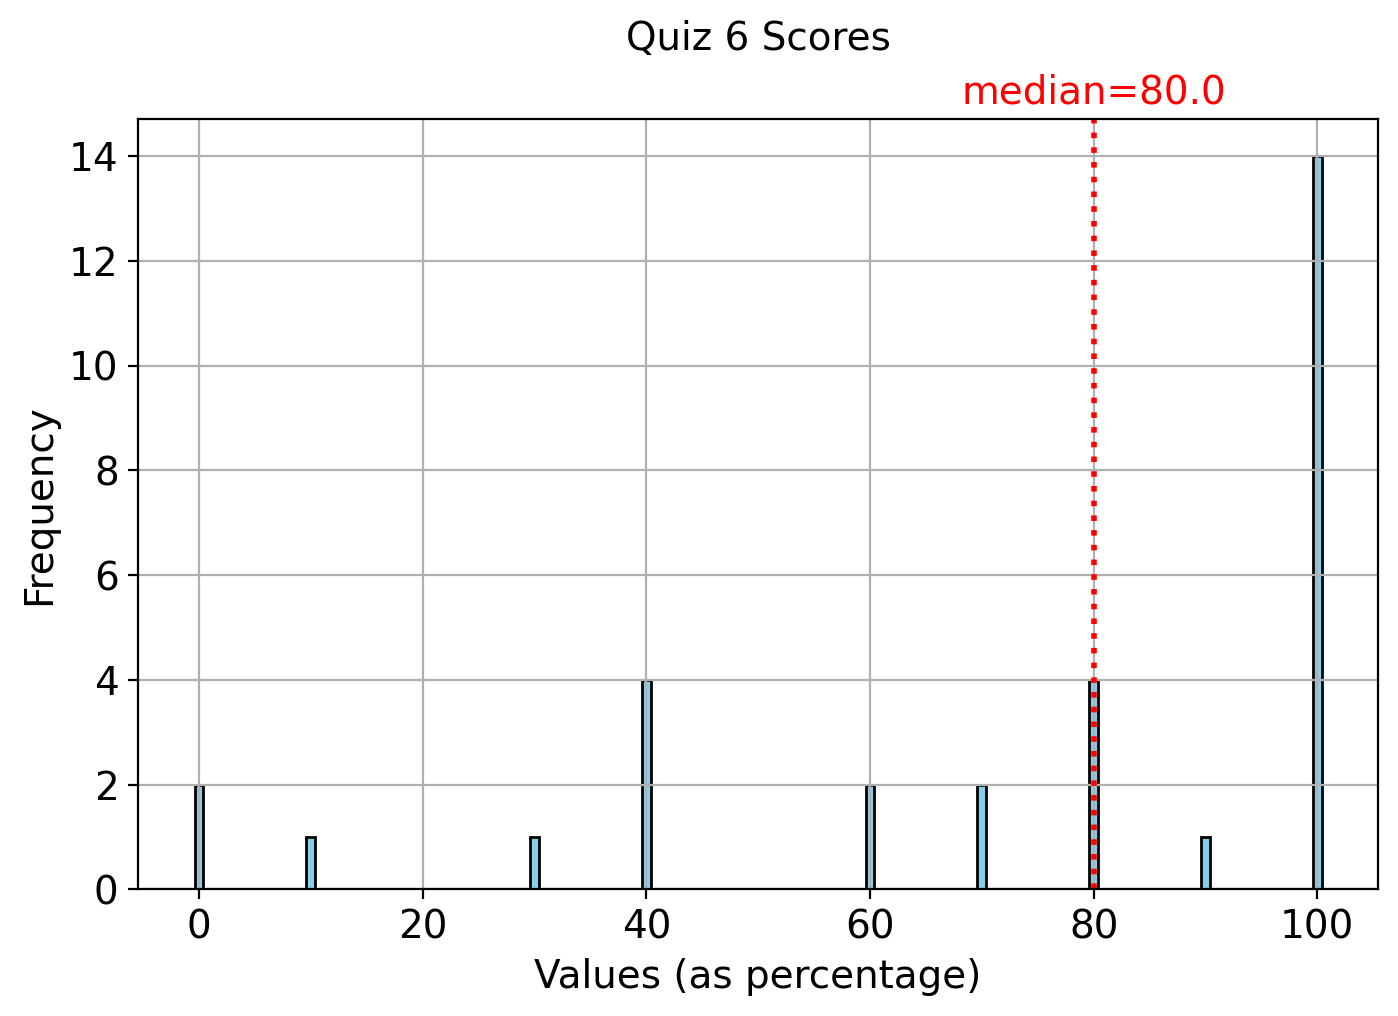
\includegraphics[width=.95\textwidth]{images/quiz_6_histogram.png}
\end{figure}
%
%\only<2>{\colorbox{green!30}{\textbf{Paul's comment.}} I would like to point out that this was a very good quiz, I think after the test, a lot of students figured out how to write proofs effectively. This quiz was much easier to grade, because students had good proof formatting.}

\end{frame}


\begin{frame}{Midterm Bonus Scores}
\begin{figure}
\only<1>{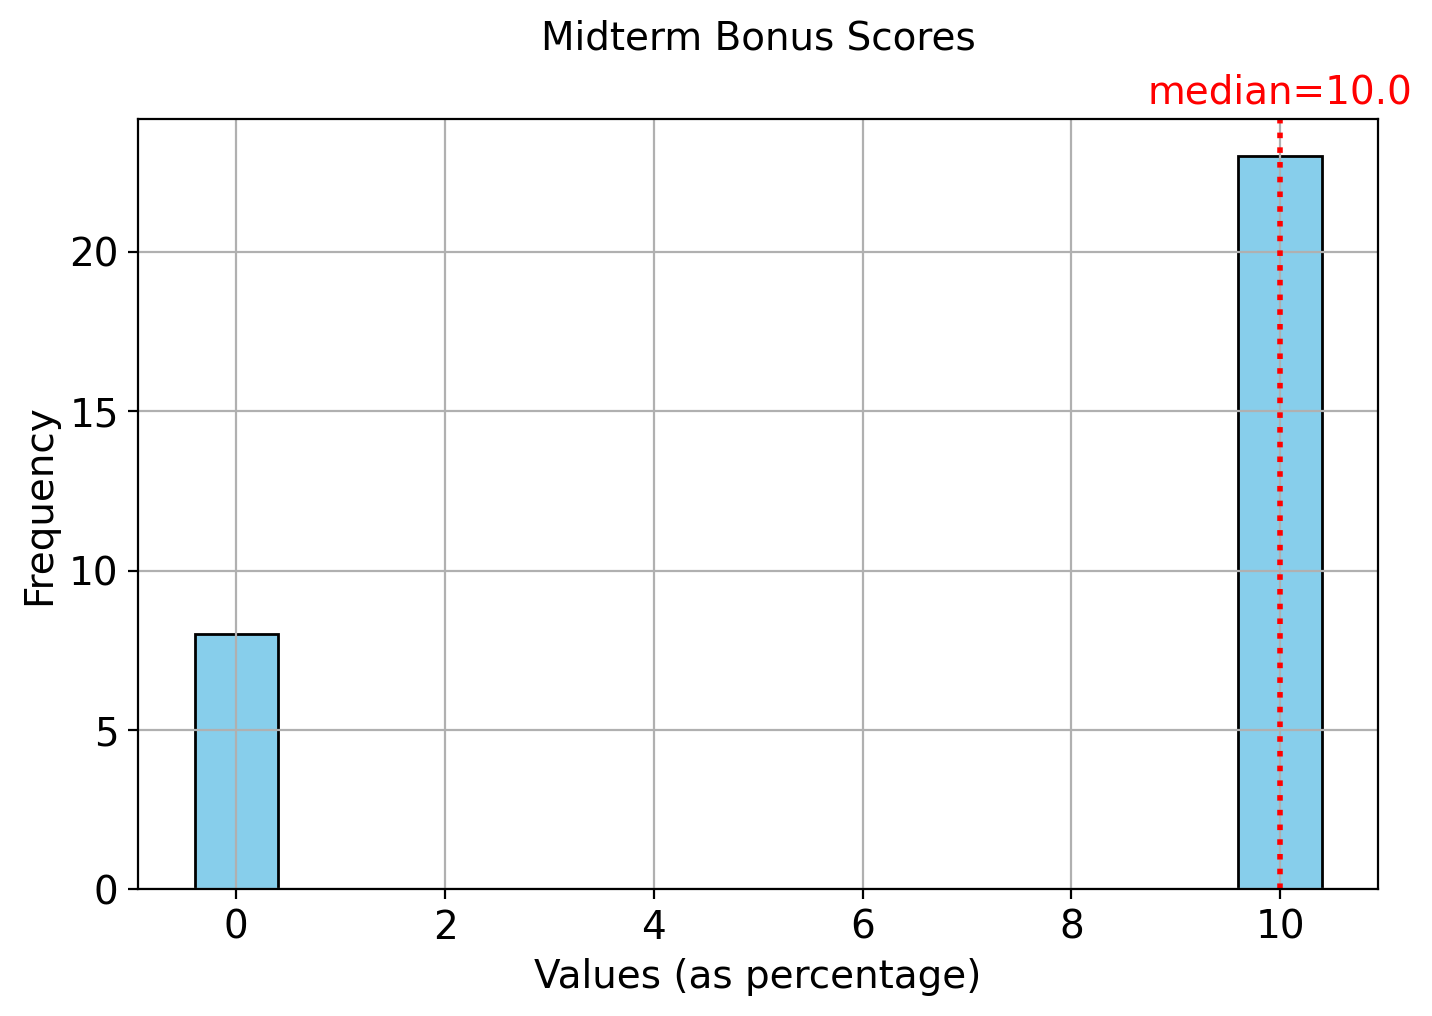
\includegraphics[width=.95\textwidth]{images/midterm_bonus_histogram.png}
}
\end{figure}

\only<2>{\begin{figure}

\includegraphics[width=\textwidth]{images/proud}
\end{figure}}
\end{frame}




\begin{frame}{Study Guide For Quiz 7}
\footnotesize 

\colorbox{yellow!20}{\textbf{Group exercises.}} Know how to solve the group exercises from the course meetings on Smallest Counterexample (10/12), Induction (10/14), and Recurrence (10/16).


\vfill 

\colorbox{red!20}{\textbf{Readings.}}  \\
\vspace{.2cm}
Sec. 21 (Smallest Counterexample)
\begin{itemize}
\item Understand Proof Templates 15 and 16 (two versions of the same thing), as used to prove Proposition 21.1.
\end{itemize}
Sec. 22 (Induction)
\begin{itemize}
\item Know how to use Theorem 22.2 / Proof Template 17 to prove Props. 22.3 and 22.5.
\item Understand the difference between Proof Template 17 and 18.
\end{itemize}
Sec. 23 (Recurrence)
\begin{itemize}
\item Know how to solve first-order recurrences from Props 23.1 and 23.3.  For example, see Example 23.2.
\item Know how to solve second-order recurrences from Theorems 23.5 and 23.9.  For example, see Example 23.6.
\item Know how to use Theorem 23.17 to find a polynomial expression to generate the first few terms of a sequence, as in Example 23.18.
\end{itemize}
\end{frame}




\agendaframe{overview}


\begin{frame}

\begin{mygreenbox}[title=Demo]
Go the nearest whiteboard and write your name  and favorite sport as follows:
\[\text{Name, Favorite sport}. \]
\tinytext{\hfill (Please write your name as your first and last name, or first name and last initial.) \hfill}	
\end{mygreenbox}


\only<2->{Let $P$ be the set of ordered pairs written on the whiteboards.}
\only<3->{Let $N$ be the names of all students in this class and $S$ be the set of all sports. \\} 



\only<4->{\colorbox{yellow!30}{\textbf{Poll.}}}
\begin{enumerate}
	\item<4-> Is $P \subseteq N \times S$? \only<5->{Is $P \subseteq S \times N$?} 
	\item<6-> Is $P$ a \alert{relation} on $N \times S$?  \only<7->{On $S \times N$?}
	\item<8-> Is $P$ a \alert{function} from $N$ to $S$?  \only<9->{From $S$ to $N$?}
\end{enumerate}

\only<10->{Let $P^{-1}$ be the set of ordered pairs obtained by reversing the entries on the whiteboard.}


\begin{enumerate}
	\item[4.]<11-> Is $P^{-1} \subseteq N \times S$? \only<12->{Is $P^{-1} \subseteq S \times N$?} 
	\item[5.]<13-> Is $P^{-1}$ a \alert{relation} on $N \times S$?  \only<14->{On $S \times N$?}
	\item[6.]<15-> Is $P^{-1}$ a \alert{function} from $N$ to $S$?  \only<16->{From $S$ to $N$?}
\end{enumerate}

	
\end{frame}

\begin{frame}{From relations to functions}
\small 
\begin{myyellowbox}[title=Poll]

Let $A=\set{1,2,3}$. Consider the relation $R$ on $A$ depicted below.

\begin{center}
\begin{tikzpicture}[scale=0.8]

% Nodes in a vertical line
\node[latent] (A1) at (-2, 2) {1};
\node[latent] (A2) at (-2, 1) {2};
\node[latent] (A3) at (-2, 0) {3};
\node[latent] (B1) at (1, 2) {1};
\node[latent] (B2) at (1, 1) {2};
\node[latent] (B3) at (1, 0) {3};


% Edges
\path[->, >=stealth] (A1) edge (B2);
\path[->, >=stealth] (A1) edge (B3);
\path[->, >=stealth] (A2) edge (B3);
\end{tikzpicture}
\end{center}
\textbf{Questions}: (1) What is a relation on $A$ in general? (2) How would you describe \underline{this} relation in words? (3) Is this relation a function?
\end{myyellowbox}

\vfill 
\pause 
\vspace{-.2cm}
\colorbox{green!30}{\textbf{Solutions.}} 
\begin{enumerate}
	\item A relation on $A$ is a subset of all pairs $(x,y)$ where $x,y \in A$.
	\only<3->{\item We have $R$ = \qq{$<$}. This is the \textbf{less than} relation.} 
	\only<4->{\item No.  A function is like a machine mapping each possible input to an output.  But here there are two problems:} \only<4>{\alert{What are they?}} \only<5->{(a) The input 3 doesn't get mapped to anything.}  \only<6->{(b) The input 1 gets mapped to 2 things.}
\end{enumerate}
\end{frame}



\begin{frame}{Functions: What are they?}

\begin{mygreenbox}[title=Definition (Hampkins pp. 128)]
We say that $f$ is \textbf{function} from $A$ to $B$, written $f : A \to B$, if $f$ is \only<1,3,4,5>{a set of pairs $ f \subseteq  A \times B$ exhibiting the \underline{function property}} \only<2>{\alert{a set of pairs $ f \subseteq  A \times B$ exhibiting the \underline{function property}}}: \only<1,2,4,5>{for every $a \in A$}\only<3>{\alert{for every $a \in A$}},  \only<1,2,3,5>{there is a unique $b \in B$ with $(a, b) \in f$}\only<4>{\alert{there is a unique $b \in B$ with $(a, b) \in f$}}. \end{mygreenbox}

\vfill 
\pause 
\begin{mybluebox}[title=Characterization]
\begin{enumerate}
	\item \only<3,4,5>{A function is a special type of a relation.}
\only<2>{\alert{A function is a special type of a relation.}}
\item We can think of a \textbf{function} as a rule that assigns  \only<2,4,5>{each element of a set $A$}\only<3>{\alert{each element of a set $A$}}\only<2,3,5>{ to \underline{exactly one} element in another set $B$.}\only<4>{\alert{ to \underline{exactly one} element in another set $B$.}}
\end{enumerate}
\end{mybluebox}
\vfill 
\only<5>{
\begin{myredbox}[title=Notation]
The object $b$ in the definition is denoted by $f(a)$ and is called the value of the function at $a$.
\end{myredbox}

}

\end{frame}




\begin{frame}

\begin{mybluebox}[title=Characterization]
We can think of a \textbf{function} as a rule that assigns each element of a set $A$ to \underline{exactly one} element in another set $B$.
\end{mybluebox}
\vfill 
\begin{myyellowbox}[title=Poll]

Let $A=\set{a,b,c,d}$ and $B=\set{e,f,g}$. Consider a relation $R$ depicted below.

\begin{center}
\begin{tikzpicture}

% Nodes in a vertical line
\node[latent] (A1) at (-2, 3) {a};
\node[latent] (A2) at (-2, 2) {b};
\node[latent] (A3) at (-2, 1) {c};
\node[latent] (A4) at (-2, 0) {d};
\node[latent] (B2) at (1, 2) {e};
\node[latent] (B3) at (1, 1) {f};
\node[latent] (B4) at (1, 0) {g};


% Edges
\path[->, >=stealth] (A1) edge (B2);
\path[->, >=stealth] (A2) edge (B2);
\path[->, >=stealth] (A3) edge (B3);
\path[->, >=stealth] (A4) edge (B2);
%\path[->, >=stealth] (A4) edge (B3);
%\path[->, >=stealth] (A4) edge (B4);
\end{tikzpicture}
\end{center}
Is $R$ a function? \pause Yes.
\end{myyellowbox}
	
\end{frame}




\begin{frame}

\begin{mybluebox}[title=Characterization]
We can think of a \textbf{function} as a rule that assigns each element of a set $A$ to \underline{exactly one} element in another set $B$.
\end{mybluebox}
\vfill 
\begin{myyellowbox}[title=Poll]

Let $A=\set{a,b,c,d}$ and $B=\set{e,f,g}$. Consider a relation $R$ depicted below.

\begin{center}
\begin{tikzpicture}

% Nodes in a vertical line
\node[latent] (A1) at (-2, 3) {a};
\node[latent] (A2) at (-2, 2) {b};
\node[latent] (A3) at (-2, 1) {c};
\node[latent] (A4) at (-2, 0) {d};
\node[latent] (B2) at (1, 2) {e};
\node[latent] (B3) at (1, 1) {f};
\node[latent] (B4) at (1, 0) {g};



% Edges
\path[->, >=stealth] (A1) edge (B2);
\path[->, >=stealth] (A2) edge (B2);
\path[->, >=stealth] (A3) edge (B3);
\path[->, >=stealth] (A4) edge (B2);
\path[->, >=stealth] (A4) edge (B3);
%\path[->, >=stealth] (A4) edge (B4);
\end{tikzpicture}
\end{center}
Is $R$ a function? \pause No. Element $d$ gets mapped to \underline{both} $e$ and $f$.
\end{myyellowbox}
	
\end{frame}


\begin{frame}

\begin{mybluebox}[title=Characterization]
We can think of a \textbf{function} as a rule that assigns each element of a set $A$ to \underline{exactly one} element in another set $B$.
\end{mybluebox}
\vfill 
\begin{myyellowbox}[title=Poll]

Let $A=\set{a,b,c,d}$ and $B=\set{e,f,g}$. Consider a relation $R$ depicted below.

\begin{center}
\begin{tikzpicture}

% Nodes in a vertical line
\node[latent] (A1) at (-2, 3) {a};
\node[latent] (A2) at (-2, 2) {b};
\node[latent] (A3) at (-2, 1) {c};
\node[latent] (A4) at (-2, 0) {d};
\node[latent] (B2) at (1, 2) {e};
\node[latent] (B3) at (1, 1) {f};
\node[latent] (B4) at (1, 0) {g};



% Edges
\path[->, >=stealth] (A1) edge (B2);
\path[->, >=stealth] (A2) edge (B2);
\path[->, >=stealth] (A3) edge (B3);
%\path[->, >=stealth] (A4) edge (B2);
%\path[->, >=stealth] (A4) edge (B3);
%\path[->, >=stealth] (A4) edge (B4);
\end{tikzpicture}
\end{center}
Is $R$ a function? \pause Not from $A$ to $B$. Element $d$ does not get mapped to anything.  \pause \only<3>{\alert{Is there a way to make it a function?}} \only<4>{However, $R$ \underline{is} function from $\set{a,b,c}$ to $B$.}
\end{myyellowbox}
	
\end{frame}


\begin{frame}{Motivation: Why are we doing this?}
\footnotesize 
\begin{minipage}{0.55\textwidth}
Often people think about functions in terms of graphs.
\end{minipage}%
\hfill
\begin{minipage}{0.4\textwidth}
\centering
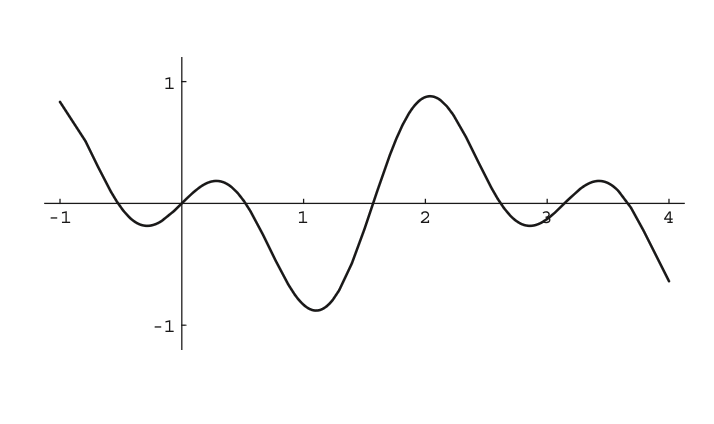
\includegraphics[width=.8\linewidth]{images/function_graph.png}
\end{minipage}
\vfill 
\pause 
\begin{mybluebox}[title=\text{However... (Quote from Scheinerman pp. 170)}]
In discrete math, we are interested in functions to and from finite sets (or $\mathbb{N}$ or $\mathbb{Z}$).  In such cases, traditional graphs of functions are either not helpful or nonsensical.
\end{mybluebox}
\vfill 
\pause 
\begin{mygreenbox}[title=\text{Example}]
Let $A$ be a finite set.   We consider the function $f: 2^A \to \mathbb{N}$ defined by $f(x) = |x|$.  \textit{(Alert: the vertical bars in this context do not mean absolute value! To each subset of $A$, the function $f$ assigns its size.)} There is no practical way to draw this as a graph on coordinate axes.
\end{mygreenbox}
\vfill \pause 
\colorbox{green!30}{\textbf{An application of the example.}} Let $A$ be  students in this class.  Then $2^A$ is the set of all subsets of students in this class. $f$ gives the number of students in each subset.  How would you plot this? \pause (Note: There are $|2^A|= 2^{51} \approx$ 1 quadrillion subsets.)
\end{frame} 





%%%% Section
\agendaframe{domain}


\begin{frame}
\footnotesize 
\begin{myyellowbox}[title=Poll]

Let $A=\set{q,r,s,t}$ and $B=\set{u,v,w}$. Consider the function below.

\begin{center}
\begin{tikzpicture}[scale=0.7]

% Nodes in a vertical line
\node[latent] (A1) at (-2, 3) {q};
\node[latent] (A2) at (-2, 2) {r};
\node[latent] (A3) at (-2, 1) {s};
\node[latent] (A4) at (-2, 0) {t};
\node[latent] (B2) at (1, 2) {u};
\node[latent] (B3) at (1, 1) {v};
\node[latent] (B4) at (1, 0) {w};


% Edges
\path[->, >=stealth] (A1) edge (B2);
\path[->, >=stealth] (A2) edge (B2);
\path[->, >=stealth] (A3) edge (B3);
\path[->, >=stealth] (A4) edge (B2);
%\path[->, >=stealth] (A4) edge (B3);
%\path[->, >=stealth] (A4) edge (B4);
\end{tikzpicture}
\end{center}


What are the domain, codomain and image? \only<2->{The domain is  $A=\set{q,r,s,t}$,}  \only<3->{ the codomain is and $B=\set{u,v,w}$,}  \only<4->{  and the image is $\set{u,v}$.}  \only<5->{Note that the image is smaller than the codomain $B$.}
\end{myyellowbox}
\vfill 
\begin{mygreenbox}[title=Definitions (Hampkins pp. 128)]
Let $f$ be a function from $A$ to $B$.  We call $A$ the \textbf{domain} of the function, and we call $B$ the \textbf{codomain} (or \textbf{target}) of the function.   \\

The \textbf{image} (or \textbf{range}) of  the function, in contrast, is the set of all elements that arise as $f(a)$ for some $a$ in the domain. (It is the set of all elements in 
$B$ that are actually \enquote{hit} by $f$).

\end{mygreenbox}
 

	
\end{frame}


%%%% Section
\agendaframe{injectivity}

\begin{frame}

\footnotesize 
\begin{mygreenbox}[title=Definitions (Hampkins pp. 128)]
%A function $f : A \to B$ is said to be  \textbf{surjective} (or \textbf{onto}) if for all $b \in B$, there is $a \in A$ such that $f(a)=b$. In other words, the range of $f$ is all of $B$. \\
A function $f : A \to B$ is said to be  \textbf{surjective} (or \textbf{onto}) if the range of $f$ is all of $B$.  (That is, all of $B$ is \enquote{hit} by the function.)\\
\vfill 
The function $f$  is said to be  \textbf{injective} (or \textbf{one-to-one}) if whenever $a \neq a'$, we have $f(a) \neq f(a')$.  (That is, distinct inputs always lead to distinct outputs.) \\
\vfill The function $f$ is said to be \textbf{bijective} if it is both surjective and injective.	
\end{mygreenbox}
 
\vfill 

\begin{myyellowbox}[title=Poll]
	\centering
	\resizebox{\textwidth}{!}{%
    \begin{tabular}{ccccc}
       \onslide<1->{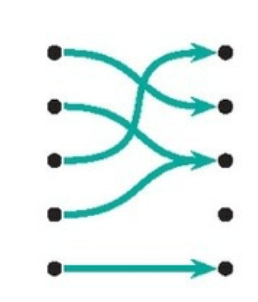
\includegraphics[width=0.2\textwidth]{images/f1.png}} & \onslide<3->{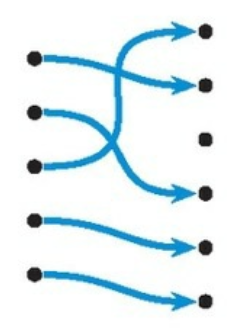
\includegraphics[width=0.2\textwidth]{images/f2.png}} & \onslide<5->{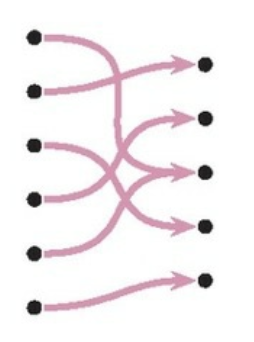
\includegraphics[width=0.2\textwidth]{images/f3.png}}  & \onslide<7->{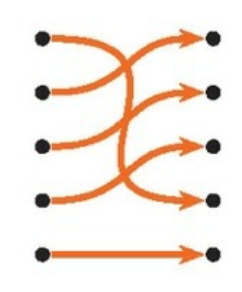
\includegraphics[width=0.2\textwidth]{images/f4.png}}  & \onslide<9->{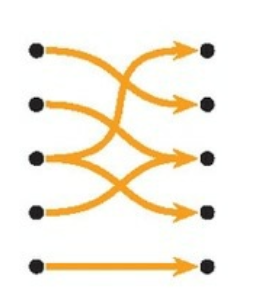
\includegraphics[width=0.2\textwidth]{images/f5.png}} \\
        \onslide<2->{Not injective} & \onslide<4->{Injective} & \onslide<6->{Not injective} & \onslide<8->{Injective} & \onslide<10->{Not a function}\\
           \onslide<2->{Not surjective} & \onslide<4->{Not surjective} & \onslide<6->{Surjective} & \onslide<8->{Surjective} & \onslide<10->{}\\
    \end{tabular}
    }
\end{myyellowbox}
\end{frame}


%%%% Section
\agendaframe{inverse}

\begin{frame}

\footnotesize 
\begin{mygreenbox}[title=Definition (Scheinerman Def. 14.4)]
Let $R$ be a relation.  The \textbf{inverse relation} of $R$, denoted $R^{-1}$, is the relation formed by reversing the order of all the ordered pairs of $R$.
\end{mygreenbox}
 
\vfill 

\begin{myredbox}[title=Theorem (Scheinerman Thm 24.21)]
Let $A$ and $B$ be sets and let $f: A \to B$.   The inverse relation $f^{-1}$ is a \textit{function} from $B$ to $A$ if and only if $f$ is a bijection.
	
\end{myredbox}
\vfill 

\begin{myyellowbox}[title=Poll]
	\centering
	\resizebox{\textwidth}{!}{%
    \begin{tabular}{ccccc}
     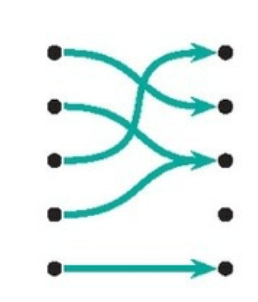
\includegraphics[width=0.2\textwidth]{images/f1.png} & 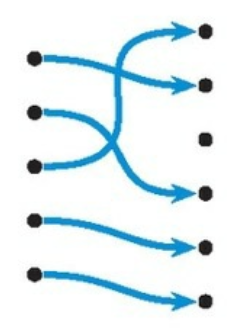
\includegraphics[width=0.2\textwidth]{images/f2.png} & 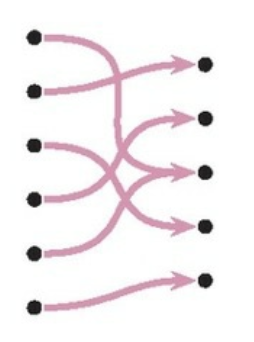
\includegraphics[width=0.2\textwidth]{images/f3.png}  & 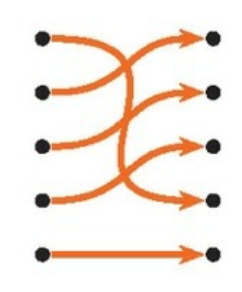
\includegraphics[width=0.2\textwidth]{images/f4.png}  & 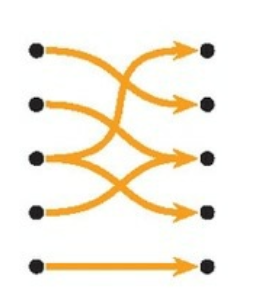
\includegraphics[width=0.2\textwidth]{images/f5.png} \\
        Not injective & Injective & Not injective & Injective & Not a function\\
           Not surjective & Not surjective & Surjective & Surjective & \\
    \end{tabular}
    } \\
    
   \vspace{0.5cm} 
For which relations $f$ above is $f^{-1}$ a function? Why or why not?
\end{myyellowbox}
\end{frame}


\begin{frame}
\small 
\begin{minipage}{0.63\textwidth}
 \begin{myyellowbox}[title=Poll]
 Let $A = \set{0,1,2,3,4}$ and $B=\set{5,6,7,8,9}$. Let $f: A \to B$ be defined by
 \[  f= \set{(0,5), (1,7), (2,8), (3,9), (4,7)}\]
 \vspace{-.25cm}
\begin{enumerate}
\item  What is  $f^{-1}$?  
\item  Is $f^{-1}$ a function from $B$ to $A$? 
\end{enumerate}
 \end{myyellowbox}
 
 \only<2->{
\colorbox{green!30}{\textbf{Solution.}}
\begin{enumerate}
	 \item<2-> $f^{-1} = \set{(5,0), (7,1), (8,2), (9,3), (7,4)}$.
	 \item<3-> No, $f$ is not bijective.  In particular:
	\begin{enumerate}
		\item<4->[a.] $f$ is not surjective.  So the input $6$ doesn't map to \textit{any} outputs.
		\item<5->[b.] $f$ is not injective.  So the input $7$ maps to \textit{multiple} outputs.
	\end{enumerate}
\end{enumerate}
}
\end{minipage}
\hfill 
\only<2->{
\begin{minipage}{0.35\textwidth}
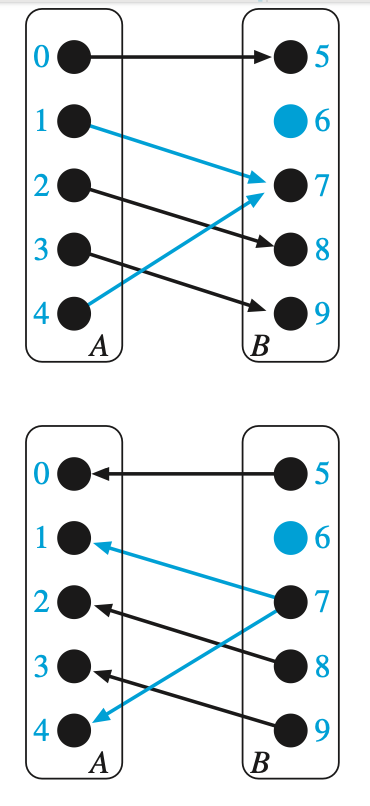
\includegraphics[width=0.8\textwidth]{images/reading_quiz_plot.png}	
\end{minipage}
}
\end{frame}


\agendaframe{applications}

\begin{frame}{Spatiotemporal fields}
\begin{figure}
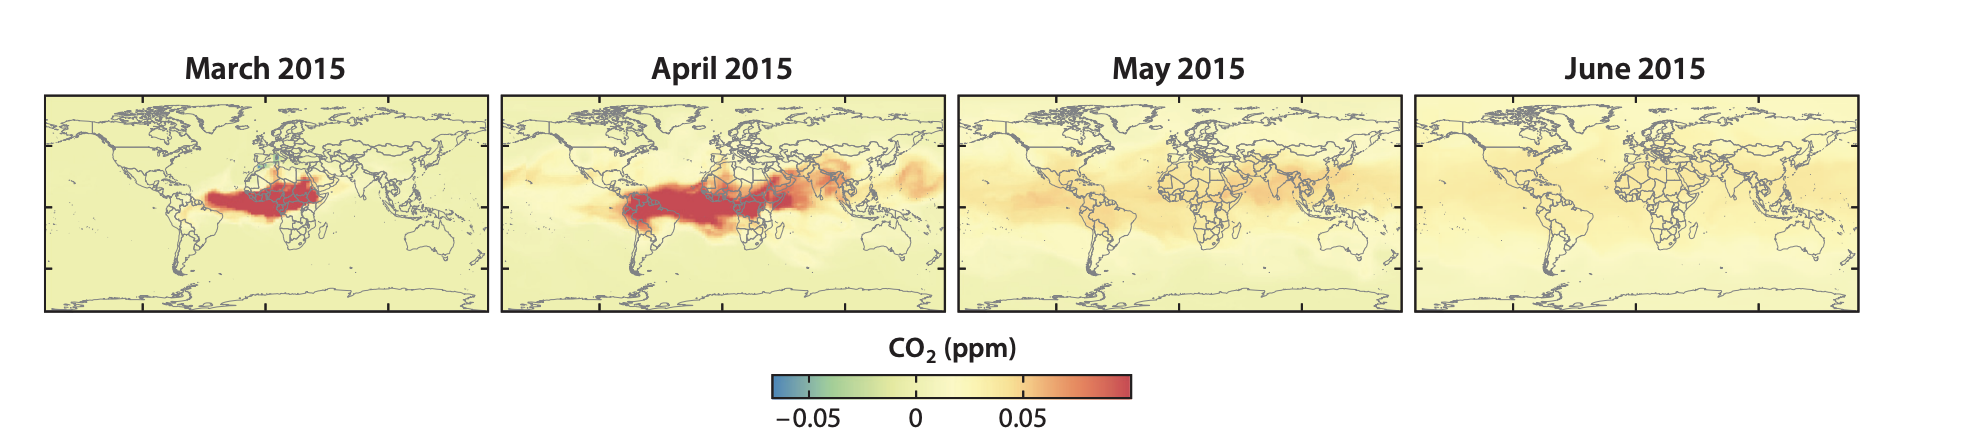
\includegraphics[width=0.95\textwidth]{images/mozart}
\caption{A spatiotemporal field showing CO2 changes, in units of parts per million (ppm), generated using the transport model MOZART.}	
\end{figure}

\pause 
\slidequote{A straightforward way to model [complicated spatial fields] is first to warp the domain. [...] More recently, a class of machine-learning models has emerged [...] where the warping is carried out using a deep neural network. [...] [One approach] circumvents [pathologies] by forcing the mapping in each layer of the deep neural network to be injective, which precludes the possibility of space-folding, where space is mapped onto itself and can create undesirable spatial-prediction artifacts}{Cressie et al. (2022), Basis-Function Models in Spatial Statistics.}
\end{frame}


\begin{frame}{Injective spatial maps}
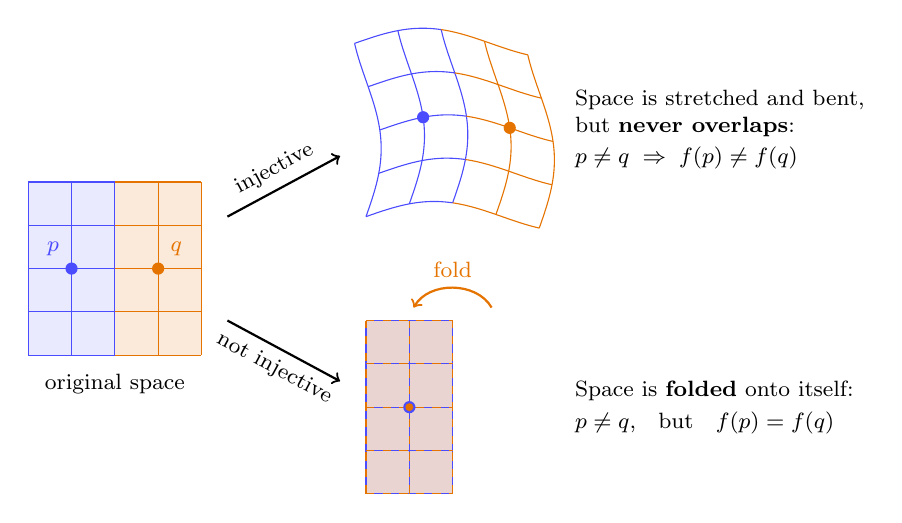
\begin{tikzpicture}[scale=0.55, every node/.style={font=\footnotesize}]
\colorlet{leftc}{blue!70}
\colorlet{rightc}{orange!90!black}

% ---------- original space (shared by both rows) ----------
\begin{scope}[shift={(0,0)}]
  \fill[leftc!12] (0,0) rectangle (2,4);
  \fill[rightc!15] (2,0) rectangle (4,4);
  \foreach \c in {0,1,2} \draw[leftc] (\c,0) -- (\c,4);
  \foreach \c in {3,4}   \draw[rightc] (\c,0) -- (\c,4);
  \foreach \c in {0,...,4} { \draw[leftc] (0,\c) -- (2,\c); \draw[rightc] (2,\c) -- (4,\c); }
  \fill[leftc]  (1,2) circle (4pt) node[above left=1pt] {$p$};
  \fill[rightc] (3,2) circle (4pt) node[above right=1pt] {$q$};
  \node[below] at (2,-0.2) {original space};
\end{scope}

% ---------- injective warp ----------
\draw[->, thick] (4.6,3.2) -- node[above, sloped] {injective} (7.2,4.6);
\begin{scope}[shift={(7.8,3.2)}]
  \foreach \c in {0,1,2} \draw[leftc, smooth, domain=0:4] plot ({\c + 0.35*sin(deg(\x))}, {\x + 0.35*sin(deg(\c))});
  \foreach \c in {3,4}   \draw[rightc, smooth, domain=0:4] plot ({\c + 0.35*sin(deg(\x))}, {\x + 0.35*sin(deg(\c))});
  \foreach \r in {0,...,4} {
    \draw[leftc,  smooth, domain=0:2] plot ({\x + 0.35*sin(deg(\r))}, {\r + 0.35*sin(deg(\x))});
    \draw[rightc, smooth, domain=2:4] plot ({\x + 0.35*sin(deg(\r))}, {\r + 0.35*sin(deg(\x))});
  }
  \fill[leftc]  ({1 + 0.35*sin(deg(2))}, {2 + 0.35*sin(deg(1))}) circle (4pt);
  \fill[rightc] ({3 + 0.35*sin(deg(2))}, {2 + 0.35*sin(deg(3))}) circle (4pt);
  \node[right, align=left] at (4.6,2) {Space is stretched and bent,\\ but \textbf{never overlaps}:\\[2pt] $p \neq q \;\Rightarrow\; f(p) \neq f(q)$};
\end{scope}

% ---------- folding (not injective) ----------
\draw[->, thick] (4.6,0.8) -- node[below, sloped] {not injective} (7.2,-0.6);
\begin{scope}[shift={(7.8,-3.2)}]
  % left half stays put; right half is folded over on top of it
  \fill[leftc!12] (0,0) rectangle (2,4);
  \fill[rightc, opacity=0.18] (0,0) rectangle (2,4);
  \foreach \c in {0,1,2} \draw[leftc] (\c,0) -- (\c,4);
  \foreach \c in {0,...,4} \draw[leftc] (0,\c) -- (2,\c);
  \foreach \c in {0,1,2} \draw[rightc, dashed] (\c,0) -- (\c,4);
  \foreach \c in {0,...,4} \draw[rightc, dashed] (0,\c) -- (2,\c);
  \draw[->, rightc, thick] (2.9,4.3) to[out=120, in=60] node[above] {fold} (1.1,4.3);
  \fill[leftc] (1,2) circle (4pt);
  \fill[rightc] (1,2) circle (2.6pt);
  \node[right, align=left] at (4.6,2) {Space is \textbf{folded} onto itself:\\[2pt] $p \neq q$, \; but \; \alert{$f(p) = f(q)$}};
\end{scope}
\end{tikzpicture}
\end{frame}

\begin{frame}[standout]
Group exercises
\end{frame}

\begin{frame}{Random group assignments}
\small 
\begin{columns}
\begin{column}{0.33\textwidth}
Ashley, Isabelle: 10 \\ 
Bailey, Tanna: 8 \\ 
Blaisdell, Olyver: 6 \\ 
Brown, Ashton: 11 \\ 
Cardenas, Dominic: 11 \\ 
Cutler, George: 1 \\ 
Fabik, Roland: 7 \\ 
Fellows, Audrey: 3 \\ 
Fitzgerald, Ryan: 5 \\ 
Fuller, Ryan: 7 \\ 
Griffen, Clara: 1 \\ 
Grutsch, Tanner: 10 \\\end{column}
\begin{column}{0.33\textwidth}
Hager, Nathan: 3 \\ 
Horner, Jayden: 12 \\ 
Johnson, Jaret: 4 \\ 
Kintzel, Samantha: 11 \\ 
Lameres, Alexis: 2 \\ 
Lee, Holden: 7 \\ 
Mayala, Reece: 9 \\ 
McLean, Connor: 3 \\ 
Mcbride, Daniel: 12 \\ 
Miller, Maverick: 4 \\ 
Moss, Emily: 12 \\ 
Mousseau, Matthew: 10 \\\end{column}
\begin{column}{0.33\textwidth}
Neuman, Evan: 8 \\ 
Putnam, John: 6 \\ 
Ramos, Vydel: 5 \\ 
Rathbun, Jedidiah: 9 \\ 
Roberts, Matthew: 6 \\ 
Roller, Nathan: 5 \\ 
Ryan, Otis: 2 \\ 
Shevtsov, Timothy: 1 \\ 
Stensland, Emma: 2 \\ 
Thiessen, Logan: 9 \\ 
Thompson, Jaiden: 4 \\ 
Vath, Ethan: 8 \\\end{column}
\end{columns}
\end{frame}


\begin{frame}{Group exercises}
\footnotesize 
\begin{enumerate}
	\item Let $A =\set{1,2,3,4}$ and $B=\set{5,6,7}$.  Let $f$ be the relation
	\[  f=\set{(1,5),(2,5), (3,6),(?,?)}\]
	Find replacements for (?,?) so that each of the following is true.
	\begin{itemize} \footnotesize 
		\item [a.] The relation $f$ is not a function from $A$ to $B$.
		\item [b.] The relation $f$ is a function from $A$ to $B$ but is not onto $B$.
		\item [c.] The relation $f$ is a function from $A$ to $B$ and is onto $B$.
	\end{itemize}
	\item For each of the following relations, answer the following questions:
	(i) Is it a function? If not, explain why and stop. Otherwise, continue onward.
	(ii) What are its domain, codomain, and image?
	(iii) Is the function injective? 
	(iv) Is it surjective?
	\begin{itemize}
	\item[a)] $\set{(x,y): x,y \in \mathbb{Z}, y=2x}$
	\item[b)] $\set{(x,y): x,y \in \mathbb{Z}, xy=0}$
	\item[c)] $\set{(x,y): x,y \in \mathbb{Z}, y=x^2}$
	\end{itemize}
	\item Let $f: \mathbb{Z} \to \mathbb{N}$ by $f(x)=|x|$.   (a) Is $f$ one-to-one? (b) Is $f$ onto?
	\item Consider the \enquote{shifting} (or translation) function $f: \mathbb{Z} \to \mathbb{Z}$ given by $f(z) = z+k$ for some fixed $k \in \mathbb{Z}$.  For instance $f(z) = z+2$ shifts all integers two units to the right.  
	\begin{itemize} \footnotesize 
		\item [a.] Prove that $f$ is a bijection.
		\item [b.] Express the inverse function $f^{-1}$ with an explicit formula.
	\end{itemize} 
\end{enumerate}
\end{frame}


\begin{frame}{Solution to group exercise \#1}
\textbf{Problem.}  Let $A =\set{1,2,3,4}$ and $B=\set{5,6,7}$.  Let $f$ be the relation
	\[  f=\set{(1,5),(2,5), (3,6),(?,?)}\]
	Find replacements for (?,?) so that each of the following is true.
	\begin{itemize} 
		\item [a.] The relation $f$ is not a function from $A$ to $B$.
		\item [b.] The relation $f$ is a function from $A$ to $B$ but is not onto $B$.
		\item [c.] The relation $f$ is a function from $A$ to $B$ and is onto $B$.
	\end{itemize}
\vfill 
\textbf{Solution.} 
	\begin{itemize} 
		\item [a.] The choice $(1,6)$ means that $1 \in A$ is related to two different elements in $B$, which is not allowed.  Moreover $4 \in A$ is not related to anything.  Note that there are many possible other solutions. [In fact, any $(x,b) \not\in \big\{(1,5),(2,5), (3,6) \big\}$  where $x \in \set{1,2,3}$ and $b \in B$ will work.]
		\item [b.] The choice $(4,5)$ means that $7 \in B$ is not \enquote{hit} by $f$.   Note that $(4,6)$ would work as well.
		\item [c.] $(4,7)$. 
	\end{itemize}

\end{frame}



\begin{frame}{Solution to Group Exercise \#2}
\footnotesize 
\textbf{Problem.} For each of the following relations, answer the following questions:
	(i) Is it a function? If not, explain why and stop. Otherwise, continue onward.
	(ii) What are its domain, codomain, and image?
	(iii) Is the function injective? 
	(iv) Is it surjective?
	\begin{itemize}
	\item[a)] $f_1 \defeq \set{(x,y): x,y \in \mathbb{Z}, y=2x}$
	\item[b)] $f_2 \defeq \set{(x,y): x,y \in \mathbb{Z}, xy=0}$
	\item[c)] $f_3 \defeq \set{(x,y): x,y \in \mathbb{Z}, y=x^2}$
	\end{itemize}
\vfill 
\textbf{Solution.}
\begin{itemize}
\item[(i)] Is it a function? $f_1$ and $f_3$ are functions because each $x$ maps to exactly one $y$.  $f_2$ is not a function because $x=0$ maps to more than one (in fact, infinitely many) $y$'s.
\item[(ii)] For all three functions, the domain and codomain are the integers. (This was explicitly stated in the problem.) The image for $f_1$ is the even integers. The image for $f_3$ is the perfect squares (i.e., $\set{0,1,4,9,\hdots}$).  
\item[(iii)] $f_1$ is injective, but $f_2$ is not.  (Think: you can recover $x$ from $y$ for $f_1$, but not $f_2$).  
\item[(iv)] $f_1$ is surjective, but $f_2$ is not.  This is immediately clear from (ii), because a function is surjective if and only if its range equals its codomain. (Think: the realized function values covers the entire space of the codomain for $f_1$, but not $f_2$.)  
\end{itemize}


\end{frame}

\begin{frame}{Solution to group exercise \#3}
\footnotesize 
\textbf{Problem.} Let $f: \mathbb{Z} \to \mathbb{N}$ by $f(x)=|x|$.   (a) Is $f$ one-to-one? (b) Is $f$ onto?
\vfill 
\textbf{Solution.}

\begin{figure}
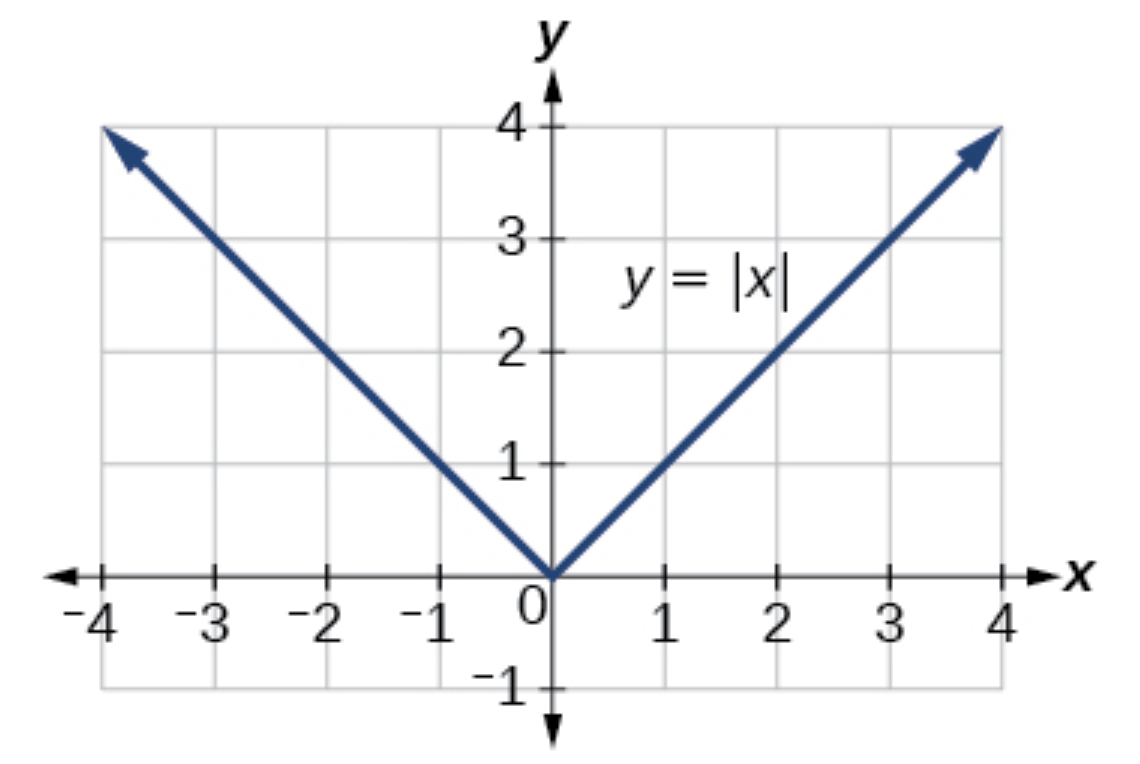
\includegraphics[width=0.5\textwidth]{images/abs_value.png}	
\end{figure}

	\begin{itemize} \footnotesize  
		\item [a.] No. For example, $f(1) = f(-1) = 1$.  Hence, distinct inputs map to the same output.
		\item [b.] Yes.  Recall that $\mathbb{N} \defeq \set{0,1,2,3, \hdots}$. We can see from the plot that all of $\mathbb{N}$ is \enquote{hit} by $f$.  For a more formal argument, we need to show that for each $n \in \mathbb{N}$, there is a $z \in \mathbb{Z}$  such that $f(z)=n$. This is easily satisfied by taking $z=n$ (or, for that matter $z=-n$).
	\end{itemize}

\end{frame}


\begin{frame}{Solution to group exercise \#4}
\footnotesize 
\textbf{Problem.} Consider the \enquote{shifting} (or translation) function $f: \mathbb{Z} \to \mathbb{Z}$ given by $f(z) = z+k$ for some fixed $k \in \mathbb{Z}$.  For instance $f(z) = z+2$ shifts all integers two units to the right.   (a) Prove that $f$ is a bijection. (b) Express the inverse function $f^{-1}$ with an explicit formula.  
%	\begin{itemize} \footnotesize 
%		\item [a.] Prove that $f$ is a bijection.
%		\item [b.] Express the inverse function $f^{-1}$ with an explicit formula.
%	\end{itemize} 
\vfill
\textbf{Solution.}
\vspace{-0.2cm}
	\begin{itemize} \footnotesize 
		\item [a.] To show that $f$ is a bijection, we need to show that it is injective and surjective.
		\begin{itemize} \footnotesize 
		\item \boxed{\text{Injective.}}  By definition, a function $f$ is injective if $a \neq a'$ implies $f(a) \neq f(a')$.  We verify this statement by contraposition. That is, we prove the logically equivalent statement that $f(a) = f(a')$ implies $a =a'$. Now 
		\[f(a) = f(a') \implies a+k = a'+k \implies a=a'. \] 
		\item \boxed{\text{Surjective.}}  By definition, a function $f$ is surjective if for any $b$ in the codomain of the function, there is an $a$ in the domain such that $f(a)=b$.  Now note that we can obtain any $b \in \mathbb{Z}$ as $b=f(a)$ by setting $a=b-k$.
		\end{itemize} 
		\item [b.] We can define $f^{-1}$ by the mapping $f^{-1}(z) = z-k.$
	\end{itemize} 
\vfill 
\begin{myredbox}[title=Remark: Proof by contraposition]
Earlier in the course, we showed that $A \implies B$ is logically equivalent to $(\texttt{not } B) \implies (\texttt{not } A)$.  (For example, this can be shown by truth tables.)  The transformed proposition is called the \underline{contrapositive}. It may be easier to prove the contrapositive form of the statement, as we did above.
\end{myredbox}

\end{frame}

\begin{frame}[standout]
Bonus group exercises
\end{frame}

\begin{frame}{Bonus group exercise}
 Consider the \enquote{zigzag} function $f: \mathbb{N} \to \mathbb{Z}$ given by 
	\[ f(n) = 
	\begin{cases}
	\frac{n}{2}, & \text{ if $n$ is even} \\
	-\frac{n+1}{2}, & \text{ if $n$ is odd} \\
	\end{cases}
	\]
	This function \enquote{zigzags} the integers like this
	\[ 0 \to 0, 1 \to -1, 2 \to 1, 3 \to -2, \hdots \]
	Prove that $f$ is a bijection.
\end{frame}

\begin{frame}{Solution (Part I) to bonus group exercise}
\scriptsize 
\begin{minipage}{0.5\textwidth}
\textbf{Problem.}  Consider the \enquote{zigzag} function $f: \mathbb{N} \to \mathbb{Z}$ given by 
	\[ f(n) = 
	\begin{cases}
	\frac{n}{2}, & \text{ if $n$ is even} \\
	-\frac{n+1}{2}, & \text{ if $n$ is odd} \\
	\end{cases}
	\]
	This function \enquote{zigzags} the integers like this
	\[ 0 \to 0, 1 \to -1, 2 \to 1, 3 \to -2, \hdots \]
	Prove that $f$ is a bijection.	
\end{minipage}
\hfill 
\begin{minipage}{0.48\textwidth}
\begin{figure}
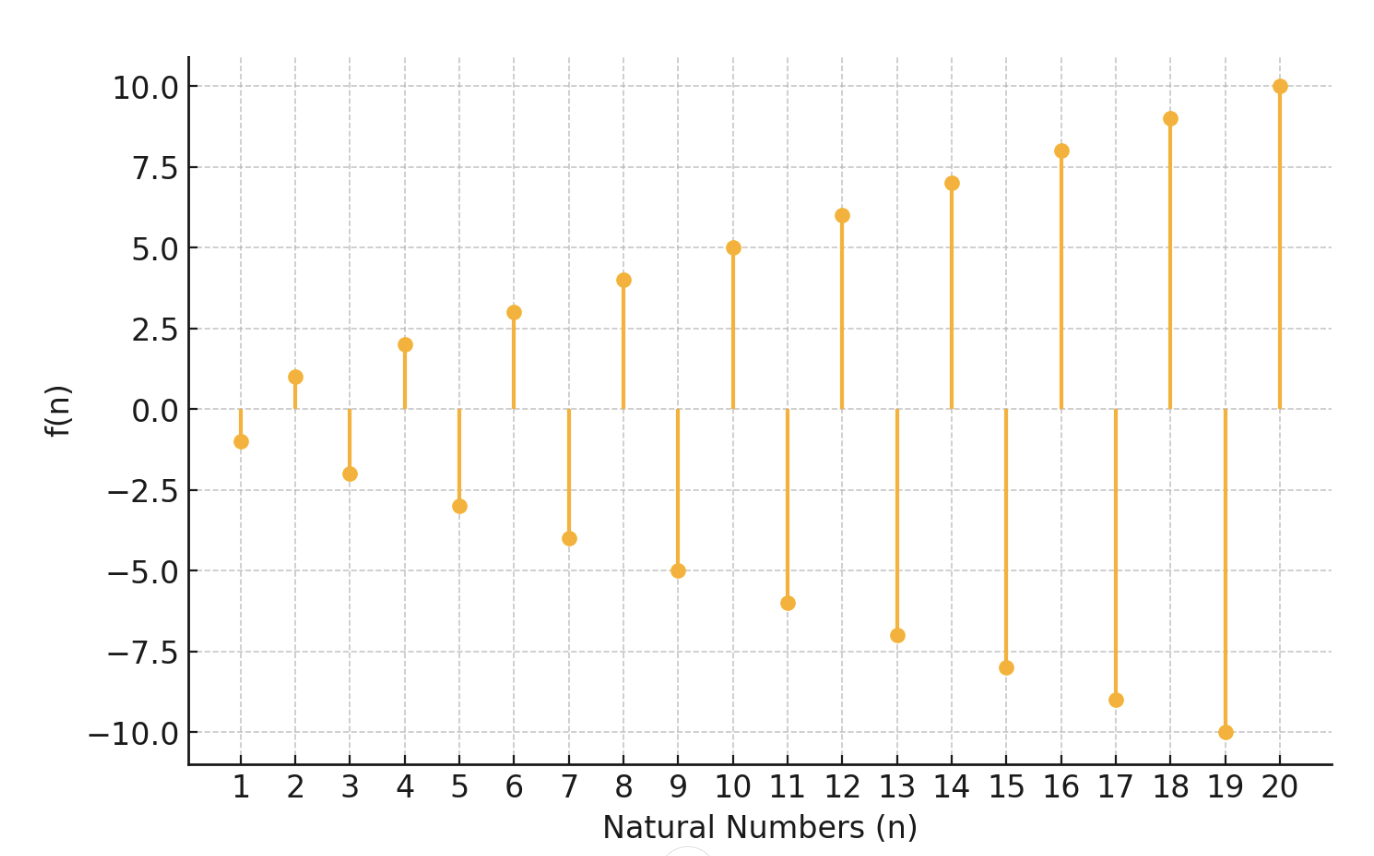
\includegraphics[width=0.95\textwidth]{images/zig_zag_function.png}	
\end{figure}
\end{minipage}
\vfill 
\textbf{Solution.}
To show that $f$ is a bijection, we need to show that it is injective and surjective.
		\begin{itemize} \scriptsize 
		\item \boxed{\text{Injective.}}  As with exercise \#3a, to prove that $f$ is injective, we show that  $f(n) = f(n')$ implies $n =n'$. First note that if $f(n)=f(n')$, then $n$ and $n'$ must have the same parity, or else $f(n)$ and $f(n')$ would have different signs.  Now
		\begin{itemize} \scriptsize 
		\item Suppose $n$ and $n'$ are both even.  Then 
		\[ f(n) = f(n') \implies \frac{n}{2} = \frac{n'}{2} \implies n=n'. \]
		\item Suppose $n$ and $n'$ are both odd.  Then 
		\[ f(n) = f(n') \implies -\frac{n+1}{2} = -\frac{n'+1}{2} \implies n=n'. \]
		\end{itemize} 
				\item \boxed{\text{Surjective.}} See next page.
		\end{itemize}
\end{frame}

\begin{frame}{Solution (Part II) to bonus group exercise}
\scriptsize 
\begin{minipage}{0.5\textwidth}
\textbf{Problem.}  Consider the \enquote{zigzag} function $f: \mathbb{N} \to \mathbb{Z}$ given by 
	\[ f(n) = 
	\begin{cases}
	\frac{n}{2}, & \text{ if $n$ is even} \\
	-\frac{n+1}{2}, & \text{ if $n$ is odd} \\
	\end{cases}
	\]
	This function \enquote{zigzags} the integers like this
	\[ 0 \to 0, 1 \to -1, 2 \to 1, 3 \to -2, \hdots \]
	Prove that $f$ is a bijection.	
\end{minipage}
\hfill 
\begin{minipage}{0.48\textwidth}
\begin{figure}
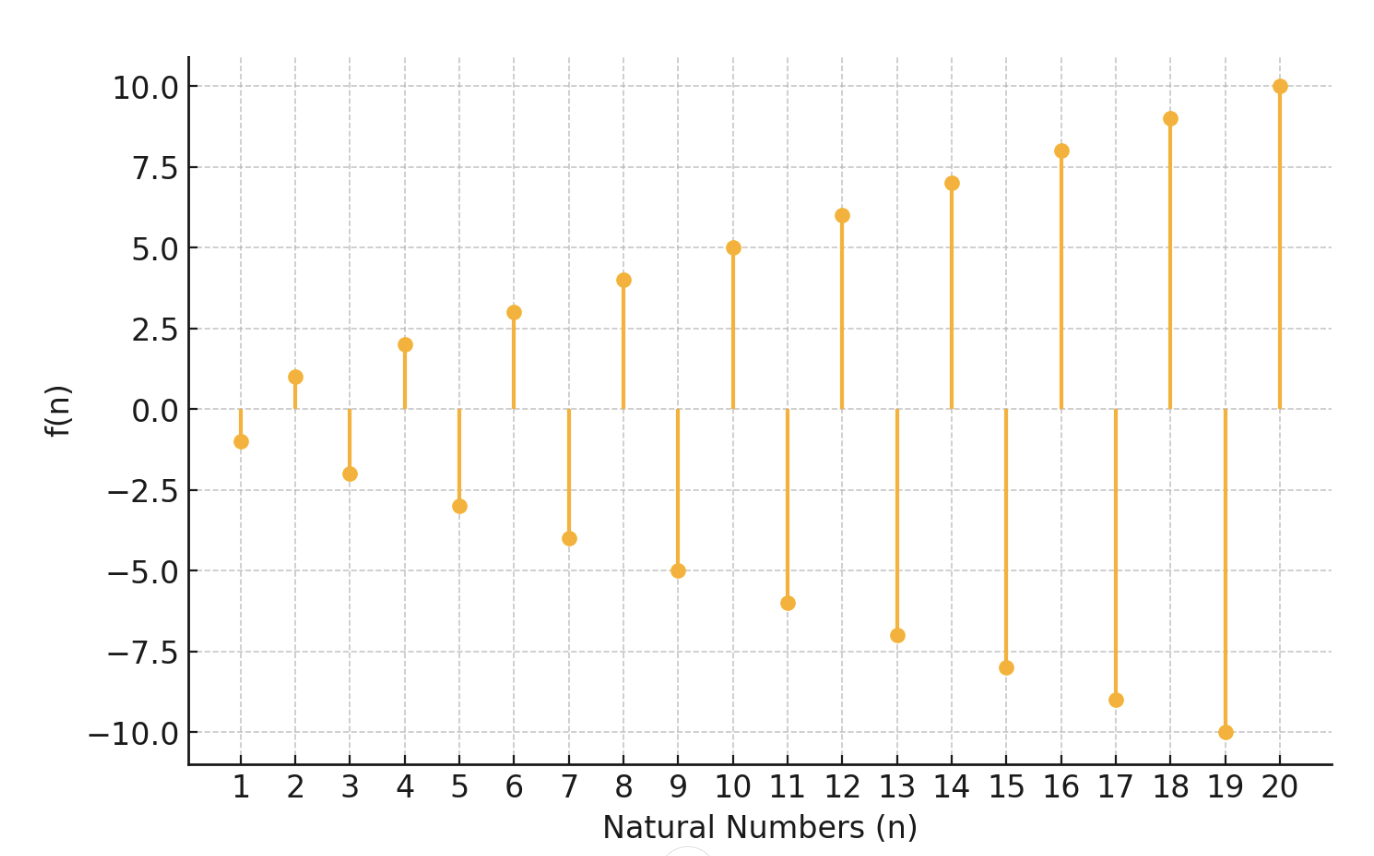
\includegraphics[width=0.95\textwidth]{images/zig_zag_function.png}	
\end{figure}
\end{minipage}
\vfill 
\textbf{Solution.}
To show that $f$ is a bijection, we need to show that it is injective and surjective.
		\begin{itemize} \scriptsize 
		\item \boxed{\text{Injective.}} See previous page.
		\item \boxed{\text{Surjective.}}  By definition, a function $f$ is surjective if for any $z \in \mathbb{Z}$, there is an $n \in \mathbb{N}$ such that $f(n)=z$.  We proceed by cases.  If $z=0$, then we take $n=0$.  If $z>0$, then we take $n=2z$.  If $z<0$, then we take $n=-2z-1$.
		\end{itemize} 
\vfill 

\begin{myredbox}[title=Remark: The strangeness of infinity]
Sets with infinitely many members have some strange properties. If $f: A \to B$ where $A$ and $B$ are finite, then $f$ being a bijection requires $|A|=|B|$.  Intuitively, each member in $A$ can't have exactly one \enquote{buddy} in $B$  unless $A$ and $B$ are the same size.  Here, however, we see that $f$ gives a bijection between $\mathbb{N}$ and $\mathbb{Z}$, even though  $\mathbb{N}$ is \enquote{smaller} than $\mathbb{Z}$ (in the sense that $\mathbb{N} \subsetneq \mathbb{Z}$).
\end{myredbox}

\end{frame}




\end{document}
